\documentclass[UTF8]{ctexart}
% 基本设置和必要宏包
\usepackage{geometry}
\geometry{a4paper,scale=0.8}

% 数学相关宏包
\usepackage{amsmath}
\usepackage{amssymb}
\usepackage{amsfonts}

\usepackage{mathtools}
\usepackage{amsbsy}
\usepackage{amstext}
\usepackage{wasysym}
\usepackage{stmaryrd}
\usepackage{mathrsfs}

% 图形和颜色
%\usepackage{xcolor}
\usepackage{graphicx}
\usepackage{subcaption}
\usepackage{caption}
\usepackage{float}

% 其他功能性宏包
\usepackage{titlesec}
\usepackage{fancyhdr}
\usepackage{setspace}
\usepackage{cite}
\usepackage{appendix}
\usepackage{listings}
\usepackage{pdfpages}
\usepackage{enumitem}
\usepackage{tabu}
\usepackage{threeparttable}
\usepackage{booktabs}
\usepackage{abstract}


\usepackage{diagbox} 

% 允许公式跨页
\allowdisplaybreaks[4]



\newcommand{\sihaoheiti}{\fontsize{14pt}\selectfont\heiti}
% 设置全局字体
%\setCJKmainfont{SimSun} % 设置正文为宋体
%\setCJKsansfont{SimHei} % 设置无衬线字体为黑体

% 论文题目设置为三号黑体字,并居中
\newcommand{\threelargebf}{\fontsize{16pt}{19.2pt}\selectfont\heiti\centering}

% 一级标题设置为四号黑体字,并居中
\titleformat{\section}{\centering\fontsize{14pt}{16pt}\bfseries\heiti}{\thesection}{1em}{}

% 二级标题设置为小四号黑体字,左对齐
\titleformat{\subsection}{\fontsize{12pt}{14.4pt}\bfseries\heiti}{\thesubsection}{1em}{\raggedright}

% 三级标题设置为小四号黑体字,左对齐
\titleformat{\subsubsection}{\fontsize{12pt}{14.4pt}\bfseries\heiti}{\thesubsubsection}{1em}{\raggedright}

% 正文字体设置为小四号宋体字,并使用单倍行距
\renewcommand{\normalsize}{\fontsize{12pt}{14.4pt}\selectfont}


%\linespread{5.0}%修改行距
% 图片文件夹
\graphicspath{{img/}}
\let\itemize\compactitem
\let\enditemize\endcompactitem

% 设置页面布局
\geometry{a4paper, left=2.5cm, right=2.5cm, top=3cm, bottom=3cm}
\setstretch{1.2}

\renewcommand{\arraystretch}{1.5}
\newcommand{\thickhline}{\noalign{\hrule height 1.2pt}} % 设置粗线的宽度
\newcommand{\thinhline}{\noalign{\hrule height 0.8pt}} % 设置细线的宽度

%%%% ===== 定理环境
\usepackage[amsmath,thref,thmmarks,hyperref]{ntheorem} % 定理宏包
%\theorempreskipamount1em % spacing before the environment
%\theorempostskipamount0em  % spacing after the environment
%\theoremstyle{plain}
%\theoremheaderfont{\normalfont\heiti}
%\theorembodyfont{\normalfont\kaishu}
%\theoremindent0em
%\theoremseparator{\hspace{0.2em}}
%\theoremnumbering{arabic}

\newtheorem{property}{性质}[section]
\newtheorem{definition}{定义}[section]
\newtheorem{lemma}{引理}[section]
\newtheorem{remark}{注记}[section]
\newtheorem{corollary}{推论}[section]
\newtheorem{example}{例}[section] 
\newtheorem{problem}{{问题}}

 \renewcommand{\abstractnamefont}{\normalfont\bfseries}  % 摘要标题字体:正常字体,粗体
\renewcommand{\abstracttextfont}{\normalfont\normalsize}     % 摘要内容字体:正常字体,小四号

% 设置页眉页脚
\pagestyle{fancy}
\fancyhf{}
\fancyfoot[C]{\thepage}
\renewcommand{\headrulewidth}{0pt}

% 设置标题格式
\titleformat{\section}{\centering\heiti\large}{\thesection}{1em}{}
\titleformat{\subsection}{\raggedright\heiti\normalsize}{\thesubsection}{1em}{}
\titleformat{\subsubsection}{\raggedright\heiti\normalsize}{\thesubsubsection}{1em}{}

% 设置摘要环境
%\newenvironment{myabstract}{
%	\begin{center}
%	\bfseries\zihao{-3} 摘要
%	\end{center}
%	\vspace{-0.5em} % 调整摘要与论文题目的距离
%	\normalsize
%}{
%}
% 设置附录环境
\renewcommand{\appendixname}{附录}
\renewcommand{\appendixpagename}{附录}

% 设置代码环境
\lstset{
	basicstyle=\small\ttfamily,
	keywordstyle=\color{blue},
	commentstyle=\color{green!70!black},
	stringstyle=\color{red},
	breaklines=true,
	numbers=left,
	numberstyle=\tiny,
	frame=tb,
	language=Python
}
\newcommand{\bbA}{\mathbb{A}}
\newcommand{\bbB}{\mathbb{B}}
\newcommand{\bbC}{\mathbb{C}}
\newcommand{\bbD}{\mathbb{D}}
\newcommand{\bbE}{\mathbb{E}}
\newcommand{\bbF}{\mathbb{F}}
\newcommand{\bbG}{\mathbb{G}}
\newcommand{\bbH}{\mathbb{H}}
\newcommand{\bbI}{\mathbb{I}}
\newcommand{\bbJ}{\mathbb{J}}
\newcommand{\bbK}{\mathbb{K}}
\newcommand{\bbL}{\mathbb{L}}
\newcommand{\bbM}{\mathbb{M}}
\newcommand{\bbN}{\mathbb{N}}
\newcommand{\bbO}{\mathbb{O}}
\newcommand{\bbP}{\mathbb{P}}
\newcommand{\bbQ}{\mathbb{Q}}
\newcommand{\bbR}{\mathbb{R}}
\newcommand{\bbS}{\mathbb{S}}
\newcommand{\bbT}{\mathbb{T}}
\newcommand{\bbU}{\mathbb{U}}
\newcommand{\bbV}{\mathbb{V}}
\newcommand{\bbW}{\mathbb{W}}
\newcommand{\bbX}{\mathbb{X}}
\newcommand{\bbY}{\mathbb{Y}}
\newcommand{\bbZ}{\mathbb{Z}}

\title{}
\author{}
\date{}

\begin{document}

\begin{titlepage}		
		
\includepdf[pages=-]{封面.pdf}
\end{titlepage}

\section{实验内容}
\begin{enumerate}
    \item 将光源置放在物屏后,打开光源,使光源透过物屏,将读数显微镜放置在光具座上,调节读数显微镜的高度,使物屏中心“1”与读数显微镜共轴,调整两者间的距离,使读数显微镜中的物象清晰,保证“1”字的拐角处最清晰。
    \item 使用显微目镜测量“1”字光源的宽度。调节叉丝,用读数显微镜读出“1”左右边缘的刻度值,分别读取三次,每次调节叉丝时不可回调(避免回程误差),计算差值,差值的平均值记为。
    \item 将物镜和目镜放置在光具座上,其中靠近物屏的是物镜,调整两个透镜之间的距离 $D$ 组成望远镜,使其分别大于或小于物镜和目镜焦距之和,以便测量不同 $D$ 下的“1”字光源像的宽度。
    \item 选用不同 $D$ 值时,改变物镜到物屏的距离 $l$分别为 $60cm$、$65cm$、$70cm$、$75cm$、$80cm$,使读数显微镜中呈现清晰的像,保证“1”拐角处最清晰。做法同上,分别读取三次,计算差值得到像宽。
    \item 将测得的数据拟合直线方程,求两方程的交点对应的像宽,所得到的物与像的比即为望远镜的放大倍数 $M$
\end{enumerate}

\begin{figure}[H]  %h此处,t页顶,b页底,p独立一页,浮动体出现的位置
		\centering
		\includegraphics[width=0.8\textwidth,height=0.5\textwidth]{img/望远镜光路图.jpg}
		%\caption{}
		\label{fig:side:b} 
\end{figure}


\section{原始数据}

\begin{table}[H]
\centering
\caption{改变物镜与目镜之间的距离测量像宽}
\begin{minipage}{0.47\linewidth}
\centering
\caption*{距离为25cm 时得到的刻度(左表)}
\begin{tabular}{c|c|c|c|c|c|}
\toprule[1pt]
\midrule
距离$l$  & 60 & 65 & 70 & 75 & 80 \\
\midrule
右刻度 &  4.625 & 4.065 & 4.011 & 3.972& 3.900\\
左刻度 &  5.310 & 4.553 & 4.485 & 4.432 & 4.282\\
\midrule
右刻度 & 4.615 & 4.098 & 4.040 & 3.987 & 3.865 \\
左刻度 & 5.312 & 4.583 & 4.514 & 4.431 & 4.261 \\
\midrule
右刻度 & 4.617 & 4.052 & 4.050 & 3.972 & 3.892 \\
左刻度 & 5.308 & 4.547 & 4.521 &  4.423 & 4.296 \\
\midrule
\bottomrule[1pt]
\end{tabular}
\end{minipage}%
\hspace{0.05\linewidth} % 可调整间距
\begin{minipage}{0.46\linewidth}
\centering
\caption*{距离为32cm 时得到的刻度(右表)}
\begin{tabular}{c|c|c|c|c|c}
\toprule[1pt]
\midrule
距离$l$ & 60 & 65 & 70 & 75 & 80 \\
\midrule
右刻度 &  4.265 & 4.025 & 3.920 & 3.937 & 3.968\\
左刻度 &  4.985 & 4.772 & 4.690 & 4.729 & 4.781\\
\midrule
右刻度 & 4.252 & 4.024 & 3.902 & 3.925 & 4.002\\
左刻度 & 4.981 & 4.773 & 4.668 & 4.822 & 4.813\\
\midrule
右刻度 & 4.266 & 4.065 & 3.921 & 3.920 & 3.971\\
左刻度 & 4.977 & 4.762 & 4.681 & 4.722 & 4.783\\
\midrule
\bottomrule[1pt]
\end{tabular}
\end{minipage}
\begin{tablenotes}
\centering
    \footnotesize
    \item[*] *上述距离单位为 $cm$,刻度单位为 $mm$
\end{tablenotes}
\end{table}



\begin{table}[H]
    \centering
    \caption{测量像宽大小}
    \begin{tabular}{c|c|c|c}
    \toprule[1pt]
       组别  &   右边缘 & 左边缘 & 差值 \\
    \midrule
       1  &  1.661 & 4.692 & 3.031 \\
    \midrule
       2  & 1.780  & 4.800 & 3.020 \\
    \midrule
       3  & 1.919 & 4.910 & 2.991 \\
    \bottomrule[1pt]
    \end{tabular}
\end{table}
\begin{tablenotes}
\centering
    \footnotesize
    \item[*] *上述刻度单位、差值单位均为 $mm$,
\end{tablenotes}

\newpage


\section{数据处理与分析}
\subsection{拟合直线方程并求放大倍数}
结合原始数据得到的其差值 $\Delta l_i$ 的数据如下表格,并利用公式 $\overline{\Delta l_i} = \frac{\sum_{i=1}^{3}}{3}$计算得到均值如下表

\begin{table}[H]
\centering
\caption{改变物镜与目镜之间的距离测量像宽}
\begin{minipage}{0.485\linewidth}
\centering
\caption*{距离为25cm 时得到的像宽(左表)}
\begin{tabular}{c|c|c|c|c|c|}
\toprule[1pt]
\midrule
距离$l$  & 60 & 65 & 70 & 75 & 80 \\
\midrule
差值  & 0.685 & 0.488 & 0.470 & 0.460 & 0.382\\
\midrule
差值  & 0.697 & 0.485 & 0.474 & 0.444 & 0.396 \\
\midrule
差值  & 0.691  & 0.495 & 0.471 & 0.451  &  0.404\\
\midrule
均值  & 0.691 & 0.4893 & 0.471 & 0.4517 & 0.394\\
\midrule
\bottomrule[1pt]
\end{tabular}
\end{minipage}%
\hspace{0.05\linewidth} % 可调整间距
\begin{minipage}{0.40\linewidth}
\centering
\caption*{距离为32cm 时得到的像宽(右表)}
\begin{tabular}{c|c|c|c|c|c}
\toprule[1pt]
\midrule
距离$l$  & 60 & 65 & 70 & 75 & 80 \\
\midrule
差值  & 0.720 & 0.747 & 0.770 & 0.792 & 0.813 \\
\midrule
差值  & 0.729 & 0.749 & 0.766 & 0.797 & 0.811 \\
\midrule
差值  & 0.721 & 0.757 & 0.760 & 0.802 & 0.812 \\
\midrule
均值  & 0.723 & 0.751 & 0.7653 & 0.797 & 0.812 \\
\midrule
\bottomrule[1pt]
\end{tabular}
\end{minipage}
\begin{tablenotes}
\centering
    \footnotesize
    \item[*] *上述距离单位为 $cm$,刻度单位为 $mm$
\end{tablenotes}
\end{table}


\begin{figure}[H]  %h此处,t页顶,b页底,p独立一页,浮动体出现的位置
		\centering
		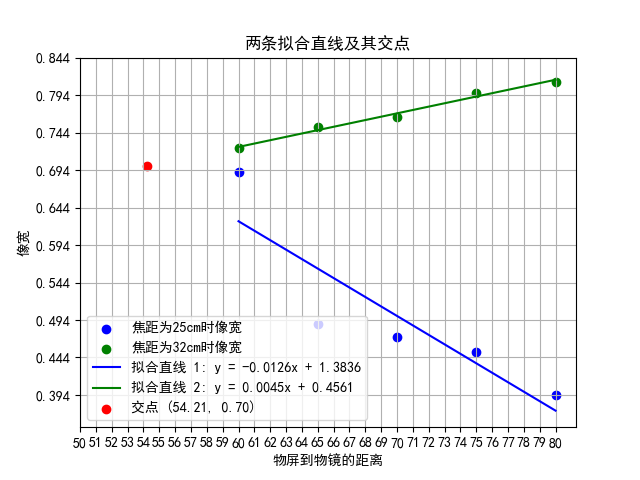
\includegraphics[width=0.7\textwidth,height=0.5\textwidth]{img/两条直线方程及其交点1.png}
		%\caption{}
		\label{fig:side:b} 
\end{figure}

设拟合得到的直线方程表达式为$W_1 = k_1l+b_1$、$W_2 = k_2l+b_2$。使用 $Python$ 运用最小二乘法拟合得到的直线方程如图所示,运用 $Python$ 进行数据处理得到拟合的直线方程表达式为 $W_1 = -0.0126l+1.3836$、$W_2 = 0.0045l+ 0.4561$,并求得交点坐标为 $(54.3064,0.6989)$

已知实验室中配备的目镜焦距 $f_0$ 为 $5cm$,物镜焦距 $f_1$ 为 $25cm$,焦距之和 $f_0 + f_1 =30 cm$
同时根据上述数据求得 “1”字光源宽度为 $\overline{d_1} = 3.0137 mm$

结合交点坐标像宽 $d_2$ 为 $0.6989 mm$,代入公式

\begin{align*}
    M = \frac{d_1}{d_2} = \frac{3.0137}{0.6989} = 4.312 
\end{align*}


\subsection{计算放大倍数的不确定度}
\subsubsection{计算测量像宽的合成标准不确定度}
已知 
\begin{align*}
    u_A(d_1) &= \sqrt{\frac{\sum_{i=1}^{3} (d_1(i) - \overline{d_1})^2}{3\times 2 }} \\
     &= \sqrt{\frac{
     (3.031 - 3.0137)^2  +   (3.020 - 3.0137)^2     +    (2.991 - 3.0137)^2
     }
     {6}
     } = 0.01193
\end{align*}
假设误差均匀分布,已知读数显微镜分度值为 $0.01mm$
\begin{align*}
    u_B(d_1) = \frac{0.01}{\sqrt{3}} \ mm  = 0.00577 \ mm
\end{align*}
综上得到合成标准不确定度如下:
\begin{align*}
    u_c(d_1) &= \sqrt{
    u_A(d_1)^2 + u_B(d_1)^2
    } \\
    &=  \sqrt{0.01193^{2}+0.00577^{2}}  \ mm = 0.01325 \ mm
\end{align*}

\subsubsection{计算得到交点坐标的不确定度}
测量斜率和截距的不确定度

由作图法得到的直线 $W_1$上两点坐标设为 $(x_1,y_1)$,$(x_2,y_2)$

假设实验测量误差分布均匀,已知横纵坐标的实验仪器对应分度值分别为 $\Delta x_i = 1 mm$、 $\Delta y_i = 0.01 mm$

\begin{align*}
    u(x_i) &= \frac{\Delta x_i}{\sqrt{3}} = \frac{1}{\sqrt{3}} = 0.57735 \ mm \\
    u(y_i) &= \frac{\Delta y_i}{\sqrt{3}} = \frac{0.01}{\sqrt{3}} = 0.0057735 \ mm \\
\end{align*}
得到斜率为
\begin{align*}
    k_1 = \frac{y_2 - y_1}{x_2 - x_1}
\end{align*}
取对数得到
\begin{align*}
    \ln{k_1} = \ln{(y_2 - y_1)} - \ln{(x_2 - x_1)}
\end{align*}

由不确定度传递公式
\begin{align*}
    u(L) = \sqrt{\sum (\frac{\partial L}{\partial x_i})^2u(x_i)^2 } 
\end{align*}


\begin{align*}
    \frac{u_{k_1}}{|k_1|} &= \sqrt{ 
    \Big(   \frac{\partial \ln{k} }{\partial y_2}        \Big)^2u^2(y_2)     +
    \Big(   \frac{\partial \ln{k} }{\partial y_1}        \Big)^2u^2(y_1)     +
    \Big(   \frac{\partial \ln{k} }{\partial x_2}        \Big)^2u^2(x_2)     +
    \Big(   \frac{\partial \ln{k} }{\partial x_1}        \Big)^2u^2(x_1)  
    } \\
    &= \sqrt{ 
    \Big(   \frac{1 }{y_2 - y_1}        \Big)^2u^2(y_2)     +
    \Big(   \frac{-1 }{y_2 - y_1}        \Big)^2u^2(y_1)     +
    \Big(   \frac{-1 }{x_2 - x_1}        \Big)^2u^2(x_2)     +
    \Big(   \frac{1 }{x_2 - x_1}        \Big)^2u^2(x_1)  
    }
\end{align*}

由于截距 $b_1 = W_1 - k_1l$
由不确定传递公式得到

\begin{align*}
    u_{b_1} = \sqrt{
    k_1^2u^2(x_2) +
    u^2(y_2) +
    x_2^2u^2_{k_1}
     }
\end{align*}

得到 $u_{k_1} = 0.01042$,$u_{b_1} = 0.10424$

同理得到 $W_2$ 上两个点坐标 $(x_3,y_3)$,$(x_4,y_4)$

\begin{align*}
    \frac{u_{k_2}}{|k_2|} &= \sqrt{ 
    \Big(   \frac{\partial \ln{k_2} }{\partial y_4}        \Big)^2u^2(y_4)     +
    \Big(   \frac{\partial \ln{k_2} }{\partial y_3}        \Big)^2u^2(y_3)     +
    \Big(   \frac{\partial \ln{k_2} }{\partial x_4}        \Big)^2u^2(x_4)     +
    \Big(   \frac{\partial \ln{k_2} }{\partial x_3}        \Big)^2u^2(x_3)  
    } \\
    &= \sqrt{ 
    \Big(   \frac{1 }{y_4 - y_3}        \Big)^2u^2(y_4)     +
    \Big(   \frac{-1 }{y_4 - y_3}        \Big)^2u^2(y_3)     +
    \Big(   \frac{-1 }{x_4 - x_3}        \Big)^2u^2(x_4)     +
    \Big(   \frac{1 }{x_4 - x_3}        \Big)^2u^2(x_3)  
    }
\end{align*}

同理截距 $b_2 = W_2 - k_2l$
\begin{align*}
    u_{b_2} = \sqrt{
    k_2^2u^2(x_4) +
    u^2(y_4) +
    x_4^2u^2_{k_2}
     }
\end{align*}

代入得到 $u_{k_2} = 0.01990  $,$u_{b_2} = 0.19897 $

已知当 $k_1 \le k_2$ 时 交点坐标 $(x_0,d_2)$ 的纵坐标为

\begin{align*}
    d_2 = \frac{k_1 b_2 - k_2 b_1}{k_1 - k_2}
\end{align*}

由不确定度传递公式
\begin{align*}
    u_c(d_2)^2 = 
    \left( \frac{b_2 - b_1}{(k_1 - k_2)^2} \right)^2 u_{k_1}^2 +
    \left( \frac{b_1 - b_2}{(k_1 - k_2)^2} \right)^2 u_{k_2}^2 +
    \left( -\frac{k_2}{k_1 - k_2} \right)^2 u_{b_1}^2 +
    \left( \frac{k_1}{k_1 - k_2} \right)^2 u_{b_2}^2
\end{align*}

带入 $b_1$、$b_2$、$k_1$、$k_2$ 得 $u_c(d_2) = 0.71251 mm $

\subsubsection{计算放大倍数的不确定度}

已知放大倍数 $$M = \frac{d_1}{d_2}$$

由不确定度传递公式得到 

\begin{align*}
    \frac{u_M}{M} = \sqrt{\frac{u_c(d_1)^2}{d_1^2} + \frac{u_c(d_2)^2}{d_2^2} } 
\end{align*}


代入 $u_c(d_1)$、$u_c(d_2)$、$d_1$、$d_2$ 得到 $u_M =  0.43960$

扩展不确定度 取置信概率 $p = 0.955$,$K_p = 2$,则$U_M$:

\begin{align*}
    U_M = K_p u_M  = 2 \times 0.43960  =  0.8792 
\end{align*}

故综上所述  $M = 4.312 \pm 0.8792$



\section{结果分析}
经过计算得到 放大倍数 $M$ 的扩展不确定度为 $M = 4.312 \pm 0.8792$ 

已知目镜和物镜的焦距 分别为焦距 $f_0 = 5cm$, $f_1 = 25cm$,焦距之和 $f_0 + f_1 =30 cm$
放大倍率理论值为 $\frac{f_1}{f_0} = 5$

综上所述,结果不符合预期。虽然放大倍数理论值在不确定度范围内,但是由于不确定度偏差较大,说明测量过程得到的结果偏差较大,从而造成实验不确定度拟合范围偶然包括理论值

经分析原因有如下几点:
\begin{enumerate}
    \item 测量时,由于不同色光经过透镜的折射率不同,在边缘发生色散,造成对象的边缘判断不准确,造成测量误差
    \item 测量像宽时,实验设备的固定读数显微镜略微向下倾斜,造成额外的读数误差、设备误差,而这些误差并未得到记录和计算
    \item 测量过程中,由于光在人眼中有重影,导致对“1”边缘的判断不够准确,可能会造成误差
    \item 在测量过程中若破坏了读数显微镜、透镜和物屏之间的共轴关系,比如实验过程中在移动读数显微镜时,操作不慎,导致其不够水平,这是测量出的不是水平的像宽,像的上下宽度不均匀,导致对宽度的测量出现偏差,结果也会产生误差。
\end{enumerate}


\newpage

\section{思考题}
\subsection{望远镜所成像随物距的变化及成缩小实像的条件}
记物距为 $u$,像距为$v$,焦距为$f$

由公式 $$\frac{1}{u} + \frac{1}{v} = \frac{1}{f}$$
\begin{enumerate}
    \item $u > 2f,f< v < 2f$,在异侧成倒立缩小的实像
    \item $u = 2f, v = 2f$,在异侧成倒立等大的实像
    \item $f < u < 2f, v > 2f$,在异侧成倒立放大的实像
    \item $u = f,v = \infty $,不成像,成平行光
    \item $u < f$,在同侧成正立放大的虚像
\end{enumerate}

成缩小实像时,$u > v$,从而 $\frac{1}{u} < \frac{1}{v}$

\begin{align*}
    \frac{1}{f} &= \frac{1}{u} + \frac{1}{v} < \frac{2}{v}  \\
    \frac{1}{f} &= \frac{1}{u} + \frac{1}{v} > \frac{2}{u}
\end{align*}

因此 $ v < 2f, u > 2f$

当 $u \to \infty $,则 $\frac{1}{v} = \frac{1}{f} - \frac{1}{u} \to  \frac{1}{f}, v \to f$

\subsection{保证测量准确的条件}
\begin{enumerate}
    \item 将望远镜固定在稳固的支架上,减少因手持或设备晃动造成的测量不准确
    \item 在进行测量时,必须保证望远镜的成像处于最清晰的状态。使用调焦机构调节望远镜,使得观察目标达到最佳的清晰度,避免因图像模糊导致误差
    \item 在通过望远镜进行目测时,确保眼睛与目镜的光轴对齐,避免因视差引入的误差
    \item 确保光屏、物镜、目镜、读数显微镜在同一轴上,减少视线误差
    \item 注意单方向调整读数显微镜叉丝,避免空程差
\end{enumerate}
\end{document}